\documentclass{article}
\usepackage[utf8]{inputenc}
\usepackage[cm]{fullpage}
%\usepackage[]{geometry}
\usepackage[]{graphicx}
\usepackage[]{listings}
\usepackage{rotating}
\usepackage{amsmath}
\usepackage{circuitikz}
\usepackage{titlesec}
\usepackage{latexsym}
\newcommand{\HRule}{\rule{\linewidth}{0.5mm}}

\titleformat{\section}
  {\normalfont\Large\bfseries}{\thesection}{1em}{}[{\titlerule[0.8pt]}]
  
\begin{document}

\begin{titlepage}
\begin{center}
% Upper part of the page. The '~' is needed because \\
% only works if a paragraph has started.

\textsc{\LARGE Oregon State University}\\[1.5cm]

\textsc{\Large CS 534}\\[0.5cm]

% Title
\HRule \\[0.4cm]
{ \huge \bfseries Implementation Assignment 1\\[0.4cm] }

\HRule \\[1.5cm]

% Author and supervisor
\noindent
\begin{minipage}{0.4\textwidth}
\begin{flushleft} \large
\emph{Students:}\\
Trevor \textsc{Fiez}\\
Ben \textsc{McCamish}
\end{flushleft}
\end{minipage}%
\begin{minipage}{0.4\textwidth}
\begin{flushright} \large
\emph{Professor:} \\
Dr.~Xiaoli \textsc{Fern}
\end{flushright}
\end{minipage}

\vfill

% Bottom of the page
{\large October 10, 2015}

\end{center}
\end{titlepage}

\section*{Problem I}

First we can look at the gradient and loss for the training dataset, represented in Figures \ref{trainingGradient} and \ref{trainingLoss} respectively. This dataset is learning over the course of time, so eventually it should converge, most of the time. We were tasked with setting the alpha, or the learning rate, of the function. As you can see from the graphs, the loss and gradient completely diverge for values of alpha larger than 0.001 and converge at values less than that. The values shown here indicate that the optimal training rate would be $\alpha=0.001$. 

    \begin{figure}[h]
      \begin{center}
      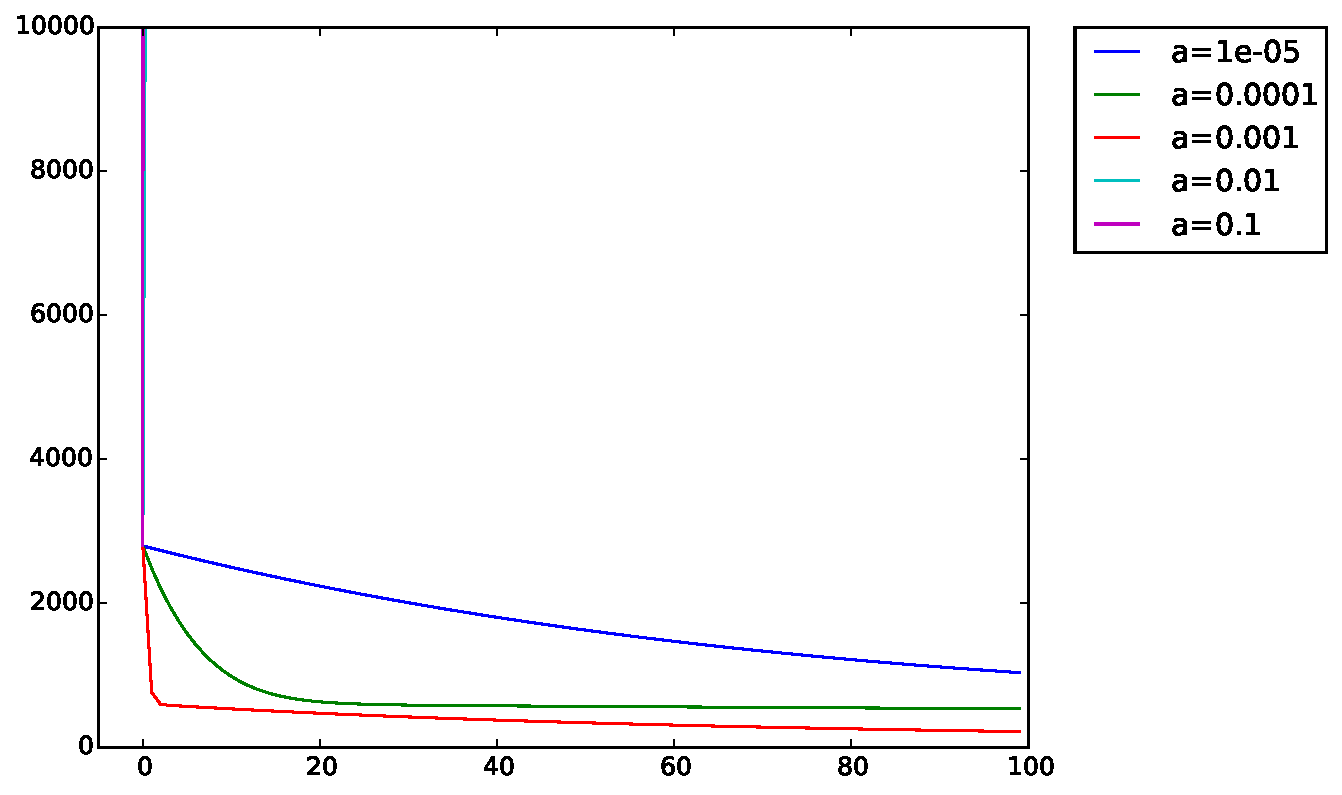
\includegraphics[scale=0.7]{trainingGradient.pdf}\\
      \end{center}
      \caption{Gradient over time for training dataset.}
      \label{trainingGradient}
    \end{figure}
    
    \begin{figure}[h]
      \begin{center}
      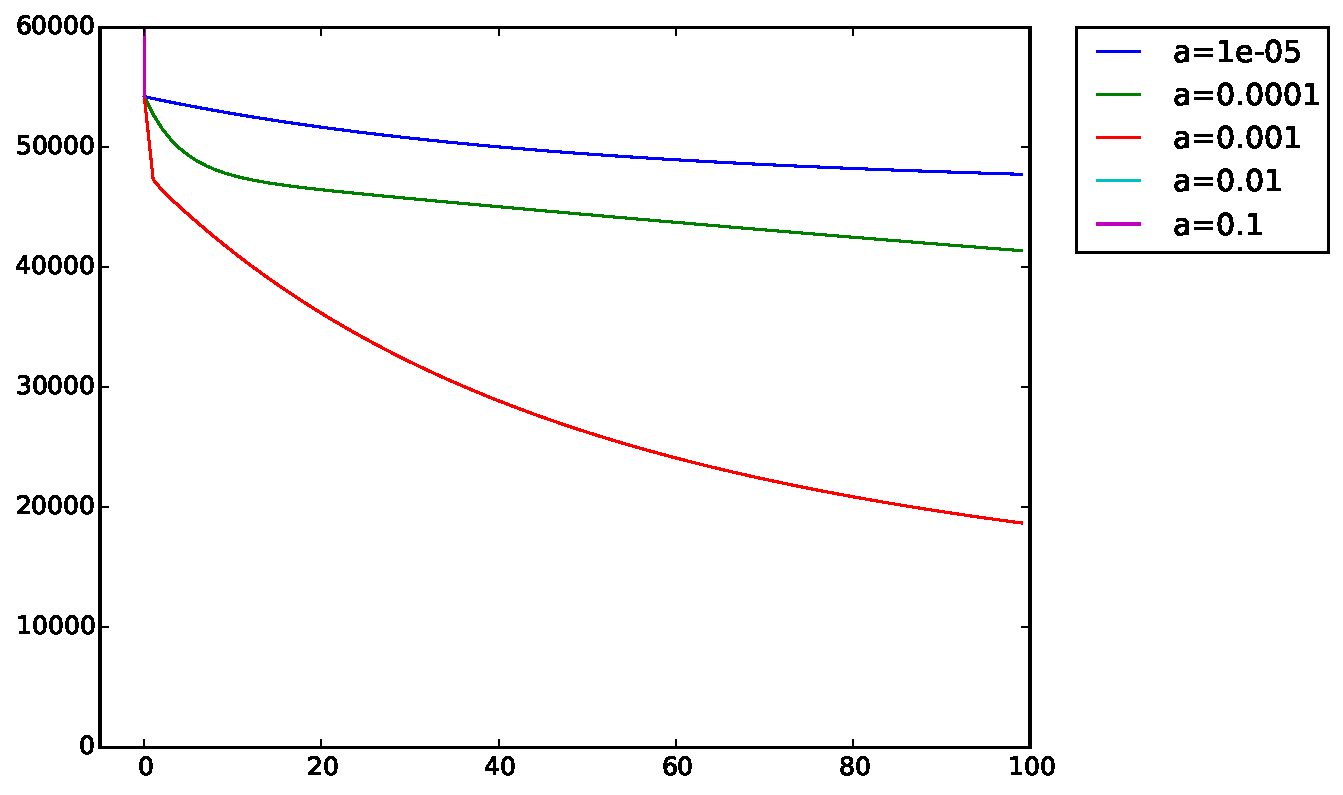
\includegraphics[scale=0.7]{trainingLoss.pdf}\\
      \end{center}
      \caption{Loss over time for training dataset.}
      \label{trainingLoss}
    \end{figure}

Figures \ref{testingLoss} and \ref{testingGradient} illustrate the gradient and loss over the testing data set. It is interesting to note, for $\alpha$ values of 0.0001 and 0.00001, the loss and gradient fluctuate much more than when $\alpha=0.001$.

    \begin{figure}[h]
      \begin{center}
      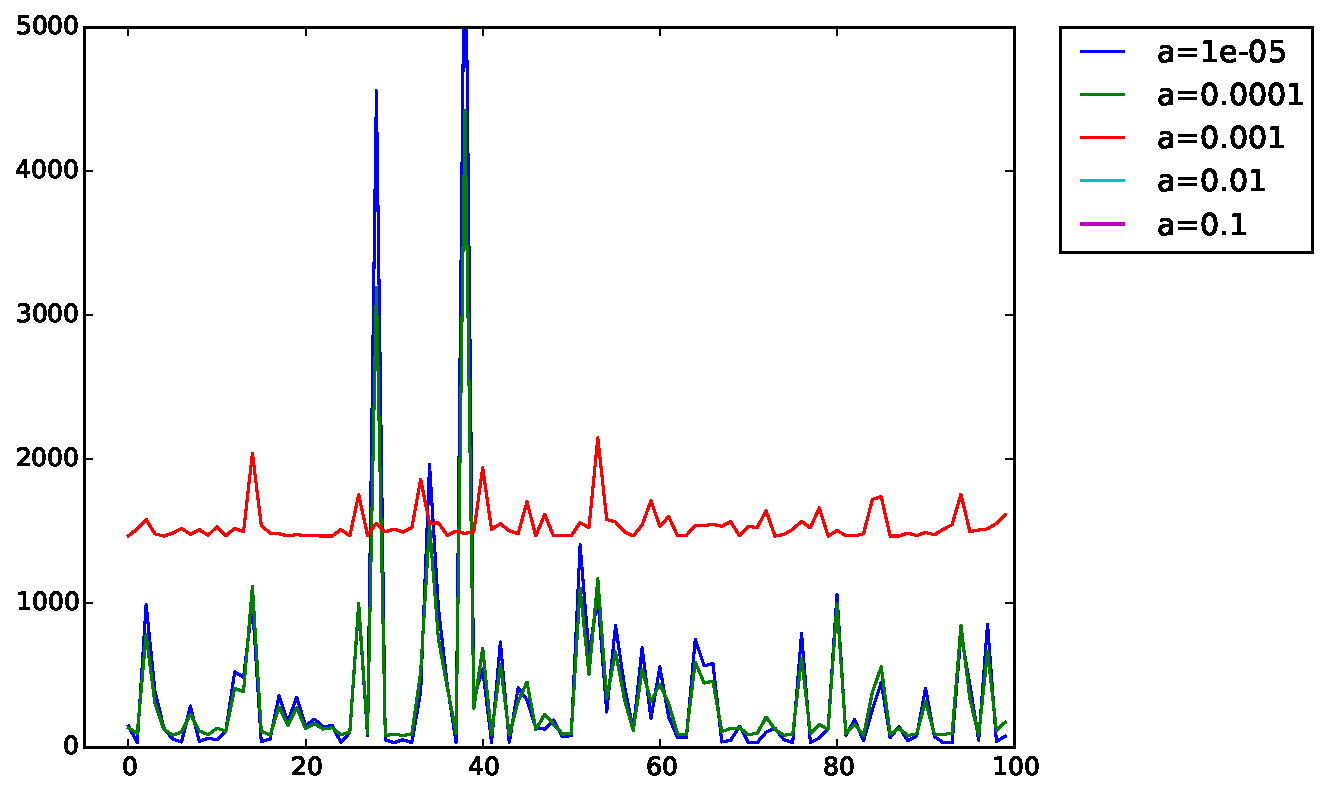
\includegraphics[scale=0.7]{testingLoss.pdf}\\
      \end{center}
      \caption{Loss over time for testing dataset.}
      \label{testingLoss}
    \end{figure}
    
    \begin{figure}[h]
      \begin{center}
      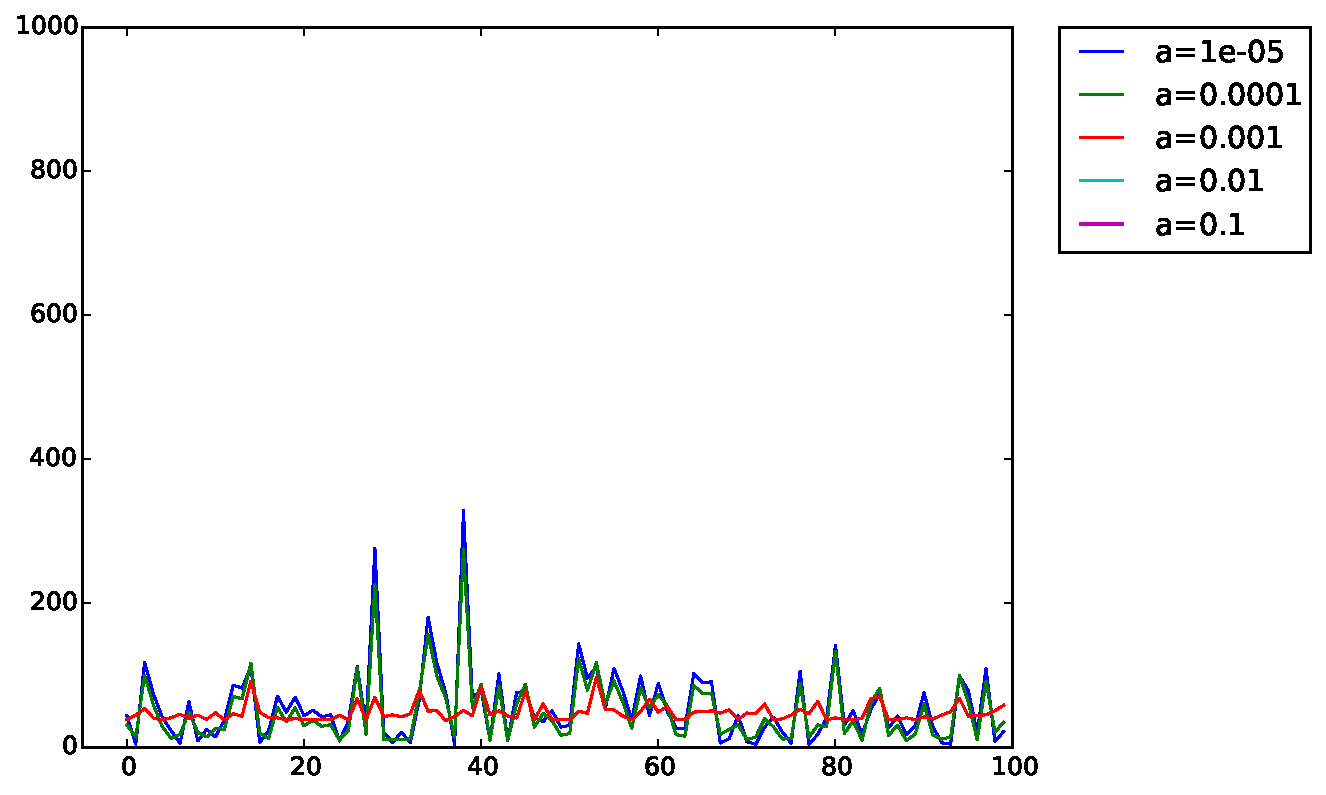
\includegraphics[scale=0.7]{testingGradient.pdf}\\
      \end{center}
      \caption{Gradient over time for testing dataset.}
      \label{testingGradient}
    \end{figure}

\section*{Problem II}
As expected, we see a concave curve in the Figure \ref{lambda}, indicating where we may experience overfitting or underfitting in the testing dataset. The training dataset has a steady increase in the SSE as the lambda increases. This may be due to the fact that gradient will be increasing since we are giving the weights too much importance, therefor ever increasing the amount of gradient we learn.
    
    \begin{figure}[h]
      \begin{center}
      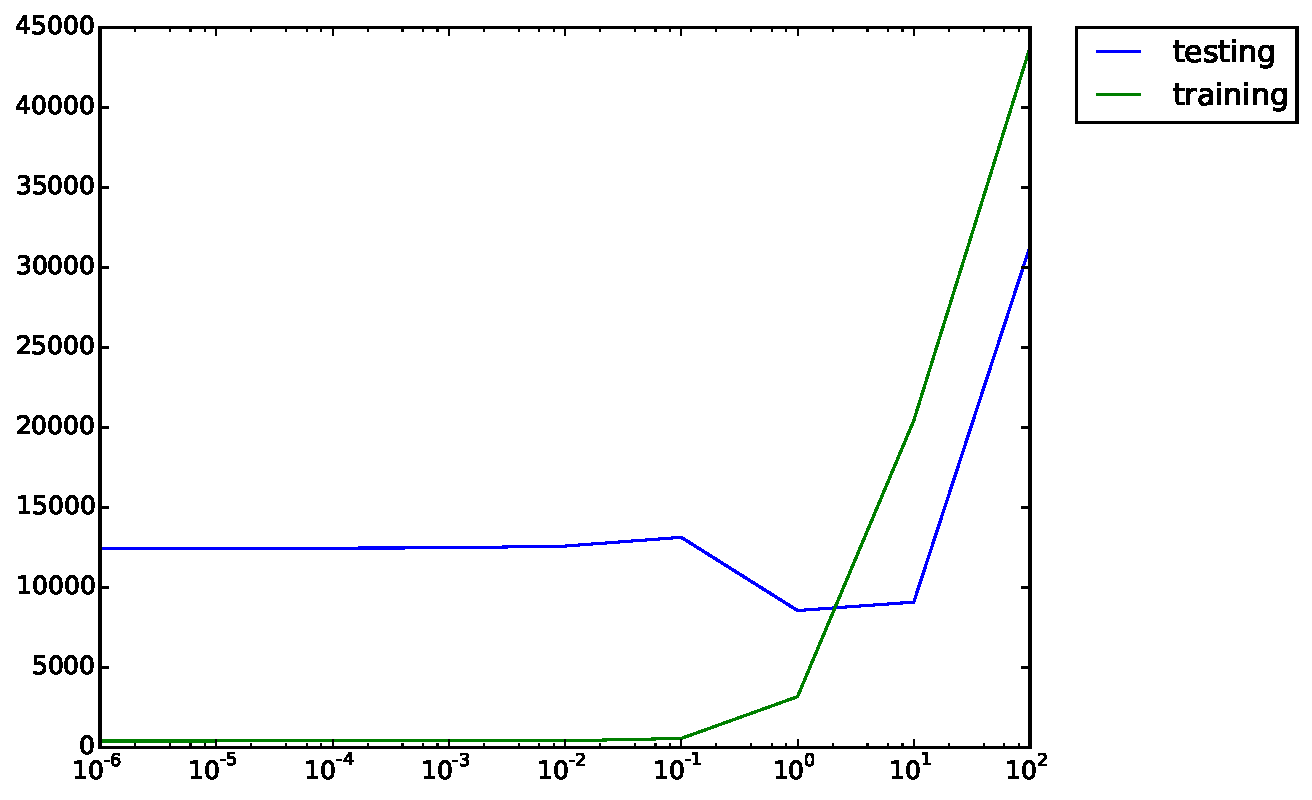
\includegraphics[scale=0.7]{SSE.pdf}\\
      \end{center}
      \caption{SSE with different lambda}
      \label{lambda}
    \end{figure}
    
    
\section*{Problem III}
\begin{enumerate}
\item 3a. I would use 0.1 as my lambda because it has the lowest loss on the testing set.

\item 3b. It is much smaller than the training SSE. The Training sum squared error is the sum over 900 examples essentially. The cross-validated SSE is only over 100 examples. So, that is partially why it is much smaller.

\item 3c. It looks extremely similar to the training SSE. It could be that the testing subsets in the cross validation are quite similar to the data we are training on. This would cause the testing SSE to resemble the training SSE because the data would be pretty much the same.
\end{enumerate}
\end{document}
